% ============================================================
% Zero- versus infinite-temperature damping in variational quantum circuits:
% output scale, spread of the expectation values, and sampling cost
% Compile: pdflatex, bibtex, pdflatex, pdflatex.
% ============================================================
\documentclass[
 aps,pra,
 twocolumn,
 superscriptaddress,
 longbibliography,
 nofootinbib
]{revtex4-2}

\usepackage{amsmath,amssymb,amsfonts,amsthm}
\usepackage{graphicx}
\graphicspath{{figures/}}
\usepackage{quantikz}
\usepackage{xcolor}
\usepackage{hyperref}
\hypersetup{colorlinks=true,linkcolor=blue,citecolor=blue,urlcolor=blue}
\usepackage{orcidlink}

\newcommand{\Tr}{\mathrm{Tr}}
\providecommand{\ket}[1]{\lvert #1 \rangle}
\providecommand{\bra}[1]{\langle #1 \rvert}
\newcommand{\AD}{\mathrm{AD}}
% Single contact address, attached to the corresponding author only.
\newcommand{\authornote}{Contact:
\href{mailto:ltkhanh@hcmus.edu.vn}{ltkhanh@hcmus.edu.vn}}

\raggedbottom
\begin{document}

\title{Zero- Versus Infinite-Temperature Damping in Variational Quantum Circuits}

\author{Vu-Quoc-Minh Nguyen\,\orcidlink{0009-0007-2748-5107}}
\affiliation{Faculty of Electronics and Telecommunications, University of Science,
Vietnam National University Ho Chi Minh City (VNU-HCM), Ho Chi Minh City 70000,
Vietnam}
\affiliation{Identity Quantum Computing JSC, 117 Tran Duy Hung Street, Hanoi 10000,
Vietnam}

\author{Tuan-Vu Truong\,\orcidlink{0009-0005-6357-6060}}
\affiliation{Identity Quantum Computing JSC, 117 Tran Duy Hung Street, Hanoi 10000,
Vietnam}

\author{Hoang-Long Nguyen\,\orcidlink{0009-0005-7922-9266}}
\affiliation{Identity Quantum Computing JSC, 117 Tran Duy Hung Street, Hanoi 10000,
Vietnam}

\author{Trung-Khanh Le\,\orcidlink{0000-0003-0935-6743}}
\thanks{\authornote}
\affiliation{Faculty of Electronics and Telecommunications, University of Science,
Vietnam National University Ho Chi Minh City (VNU-HCM), Ho Chi Minh City 70000,
Vietnam}

\date{\today}

\begin{abstract}
Randomized compiling turns amplitude damping (AD) into its Pauli twirl, which
keeps the contraction of the damping but removes its non-unital term. The twirl
is generalized amplitude damping at infinite temperature, so comparing the two
isolates the zero-temperature bias of the damping. A recent study reported that
twirling degrades variational models. It remains unclear whether this reflects
a real loss in what the models can learn or only a change in how their outputs
must be read out. In this work, we compare AD with its Pauli and Clifford
twirls in exact simulations of a re-uploading classifier. We show that the bias
acts mainly through the spread of the measured expectation values over the
inputs. Under AD, this spread settles on a floor that vanishes at infinite
temperature, whereas under the twirls it keeps shrinking with every layer. A
trainable readout recovers the noiseless accuracy under every channel. The
difference reappears instead as a cost in measurement shots. At a fixed shot
budget, the classifier under AD stays close to its noiseless accuracy, while
the twirled classifiers fall far below it. At weak damping, the two separate
only in very deep circuits.
\end{abstract}

\maketitle

% ============================================================
\section{Introduction}
\label{sec:intro}

Variational quantum algorithms and quantum machine learning models are built
from parameterized circuits and are meant to run on noisy near-term
devices~\cite{preskill2018nisq,cerezo2021variational,bharti2022noisy}. Whether
such a model can be trained depends on how strongly its outputs vary with the
parameters. In deep random circuits, this variation vanishes exponentially with
the number of qubits, a phenomenon known as a barren
plateau~\cite{mcclean2018barren,cerezo2021cost,larocca2025barren}, and noise can
make it worse. Unital noise drives the state toward the maximally mixed state,
so local expectation values decay exponentially with
depth~\cite{wang2021noiseinduced,stilckfranca2021limitations}. Non-unital noise
behaves differently. Amplitude damping (AD) drives the state toward a pure state
and avoids barren plateaus for local observables~\cite{mele2026noise}, although
the output then forgets the early
layers~\cite{schumann2024emergence,singkanipa2025beyond}.

This difference matters in practice, because hardware noise is often made
unital on purpose. Randomized
compiling~\cite{wallman2016noise,hashim2021randomized} averages the noise over
random Pauli gates, which turns AD into its Pauli twirl. The twirl keeps the
contraction of AD but removes its non-unital term, the pull toward $\ket{0}$,
and leaves generalized amplitude damping at infinite temperature. Comparing AD
with its Pauli twirl therefore isolates the zero-temperature bias of the
damping. A recent study~\cite{vanrossum2026biased} made
this comparison and found that twirling shrinks gradients and degrades the
performance of variational models. What these effects mean is less clear. They
could reflect a real loss in what the model can learn, or only a change in how
its outputs must be read out.

In this work, we show that in our classifier the zero-temperature bias acts mainly
through the spread of the measured expectation values over the inputs. Under
AD, this spread settles on a floor, whereas under the twirls it keeps shrinking
with every layer. The floor vanishes as the temperature rises. A trainable
readout absorbs most of the resulting differences in accuracy, much as
rescaling methods of error mitigation do~\cite{vovrosh2021simple}, so the
twirled models lose little in what they can learn. The difference reappears
instead as a cost in measurement shots~\cite{wang2024errormitigation}: at a
fixed shot budget, the classifier under AD stays close to its noiseless
accuracy, while the twirled classifiers fall far below it. At weak damping, the
two separate only in very deep circuits.
Together, these findings explain the reported degradation as a loss of output scale,
which a trained readout restores at a cost in shots.

We organize the text as follows. Section~\ref{sec:setting} introduces the
channels and the classifier. Section~\ref{sec:scale} treats the output scale,
and Sec.~\ref{sec:cost} the spread, the sampling cost, and their dependence on
the damping strength. Section~\ref{sec:conclusion} concludes.

% ============================================================
\section{Channels and model}
\label{sec:setting}

In this section, we introduce the noise channels that we compare and the
four-qubit re-uploading classifier on which we compare them.

\subsection{Channels}
\label{sec:channels}

We describe each single-qubit channel $\mathcal N$ through its action on the
Bloch vector, which is an affine map $\mathbf r\mapsto T\mathbf r+\mathbf t$~\cite{nielsen2010quantum}, with
\begin{equation}
T_{ij}=\tfrac12\Tr\bigl[P_i\,\mathcal N(P_j)\bigr],\qquad
t_i=\tfrac12\Tr\bigl[P_i\,\mathcal N(I)\bigr],
\label{eq:bloch}
\end{equation}
where $P_i\in\{X,Y,Z\}$. The matrix $T$ describes how the channel shrinks the
Bloch vector, and the vector $\mathbf t$ how it pushes it. The channel is
unital if and only if $\mathbf t=\mathbf 0$.

We compare amplitude damping with two twirled versions of it. Amplitude damping
of strength $p$ does two things to the Bloch vector. It shrinks the vector, by
$c=\sqrt{1-p}$ in the transverse directions and by $c^2$ along $z$, and it
pushes the vector toward $\ket0$ by $p$. The Clifford twirl~\cite{dankert2009exact}
averages these effects over all directions and leaves depolarizing noise, which
shrinks every component by the same factor and pushes nowhere. The Pauli
twirl~\cite{dur2005standard,wallman2016noise} is gentler. It keeps the
shrinking of AD exactly but removes the push toward $\ket0$, the non-unital
term.

This comparison has a simple physical meaning. Generalized amplitude
damping~\cite{nielsen2010quantum} with excited-state population $N$ has the
same $T$ as AD and $t_z=p(1-2N)$. AD is the case $N=0$, and its Pauli twirl is
the case $N=\frac12$. Comparing AD with its Pauli twirl therefore compares
damping at zero and at infinite temperature.

We treat the twirled channels as idealized, replacing the channel by its twirl
at every insertion. No twirling protocol can do this exactly after a
non-Clifford gate such as the data encoding, so the twirled channels should be
read as model channels that share the contraction of AD.

\subsection{Four-qubit re-uploading classifier}
\label{sec:model_clf}

\begin{figure*}[!t]
\centering
\begin{quantikz}[column sep=3.2pt, row sep=10pt, thin lines]
\lstick{$\ket{0}$}
 & \gate{R_Z}\gategroup[4,steps=10,style={dashed,rounded corners,
 inner xsep=3pt,inner ysep=3pt},background,
 label style={label position=below,anchor=north,yshift=-0.35cm}]
 {\small one layer, repeated $\times L$}
 & \gate{R_Y} & \gate{R_Z} & \ctrl{1} & & & \targ{}
 & \gate[4]{\mathcal N^{\otimes n}} & \gate{R_X(a_1)}
 & \gate[4]{\mathcal N^{\otimes n}}
 & \gate{R_Z} & \gate{R_Y} & \gate{R_Z}
 & \gate[4]{\mathcal N^{\otimes n}} & \meter{} & \rstick{$z_1$} \\
\lstick{$\ket{0}$}
 & \gate{R_Z} & \gate{R_Y} & \gate{R_Z} & \targ{} & \ctrl{1} & &
 & & \gate{R_X(a_2)} & & \gate{R_Z} & \gate{R_Y} & \gate{R_Z} & &
 \meter{} & \rstick{$z_2$} \\
\lstick{$\ket{0}$}
 & \gate{R_Z} & \gate{R_Y} & \gate{R_Z} & & \targ{} & \ctrl{1} &
 & & \gate{R_X(a_3)} & & \gate{R_Z} & \gate{R_Y} & \gate{R_Z} & &
 \meter{} & \rstick{$z_3$} \\
\lstick{$\ket{0}$}
 & \gate{R_Z} & \gate{R_Y} & \gate{R_Z} & & & \targ{} & \ctrl{-3}
 & & \gate{R_X(a_4)} & & \gate{R_Z} & \gate{R_Y} & \gate{R_Z} & &
 \meter{} & \rstick{$z_4$}
\end{quantikz}
\caption{The classifier at $n=4$, drawn for one layer and the final block.
Each $R_ZR_YR_Z$ triple carries three trainable angles; the encoding column
re-uploads the angle vector $\mathbf a$ in each of the $L$ layers. The channel
acts on every qubit after the entangler, after the encoding, and after the
final block, giving $2L+1$ insertions per qubit. The expectation values
$z_j=\langle Z_j\rangle$ enter a trainable affine readout.}
\label{fig:circuit}
\end{figure*}

Our model is a data re-uploading
classifier~\cite{perezsalinas2020data,schuld2021encoding} on $n=4$ qubits
(Fig.~\ref{fig:circuit}), which classifies MNIST
images~\cite{lecun1998gradient} of the digits $\{1,3,5\}$. Each image is
reduced to four principal components, which are mapped linearly to angles
$a_j\in[0,2\pi]$. As a second data set, we
use three classes of Fashion-MNIST~\cite{xiao2017fashion}.

The circuit is built from three ingredients, namely trainable blocks, the
encoding, and a ring of CNOTs,
\begin{equation}
\begin{gathered}
\mathcal R^{(\ell)}={\textstyle\bigotimes_{j=1}^{n}}R_Z R_Y R_Z,\quad
S(\mathbf a)={\textstyle\bigotimes_{j=1}^{n}}R_X(a_j),\\
E=\mathrm{CNOT}_{n,1}\cdots\mathrm{CNOT}_{2,3}\,\mathrm{CNOT}_{1,2},
\end{gathered}
\label{eq:blocks}
\end{equation}
where $\mathrm{CNOT}_{j,k}$ has control $j$ and target $k$. Each layer applies a
trainable block and the ring, then the encoding, with the channel acting after
both,
\begin{equation}
\mathcal L^{(\ell)}_{\mathbf a}=\mathcal N^{\otimes n}\circ
\mathcal U\bigl(S(\mathbf a)\bigr)\circ\mathcal N^{\otimes n}\circ
\mathcal U\bigl(E\,\mathcal R^{(\ell)}\bigr),
\label{eq:layer}
\end{equation}
and the full circuit is
\begin{equation}
\Phi_{\mathbf a,\theta}=\mathcal N^{\otimes n}\circ\mathcal U\bigl(\mathcal R^{(L)}\bigr)
\circ\mathcal L^{(L-1)}_{\mathbf a}\circ\cdots\circ\mathcal L^{(0)}_{\mathbf a},
\label{eq:circuit}
\end{equation}
with $2L+1$ insertions of the channel per qubit and $\theta$ the $3n(L+1)$
trainable angles of the blocks. The readout acts on the
single-qubit expectation values
\begin{equation}
z_j(\mathbf a,\theta)=\Tr\bigl[Z_j\,\Phi_{\mathbf a,\theta}
\bigl(\ket0\bra0^{\otimes n}\bigr)\bigr],
\label{eq:features}
\end{equation}
and the scores of the three classes are
\begin{equation}
\ell(\mathbf a)=
\begin{cases}
W\mathbf z+\mathbf b & \text{(raw)},\\
W\,\mathrm{diag}(\boldsymbol\sigma)^{-1}(\mathbf z-\boldsymbol\mu)+\mathbf b
 & \text{(standardized)},
\end{cases}
\label{eq:readout}
\end{equation}
where $W$ is a trainable $3\times n$ weight matrix and $\mathbf b$ a trainable
bias. In the standardized readout, $\boldsymbol\mu$ and $\boldsymbol\sigma$
collect the means $\mu_j$ and the population standard deviations $\sigma_j$ of
the $z_j$ over the 1000 training images. We recompute them at every
training step, with gradients flowing through them, and apply their values at
the final parameters to the test images. The standardized readout adds no
parameters to the raw one. It only fixes the scale at which $W$ acts.

Unless stated otherwise, we use $p=0.3$ and simulate the density matrix
exactly, so the expectation values carry no sampling error. The exception is
the finite-shot runs, in which each $z_j$ carries the noise of $N_s$
measurements, in training as well as at test time. For these runs, we define
the operational shot cost of a trained model as the smallest $N_s$ at which its
mean test accuracy lies within 0.01 of its accuracy with exact expectation
values, and we report its geometric mean over the initializations. Training
settings, classical baselines, and the shot model are given in
Appendix~\ref{app:training}.

% ============================================================
\section{Output scale}
\label{sec:scale}

\begin{figure*}[t]
\centering
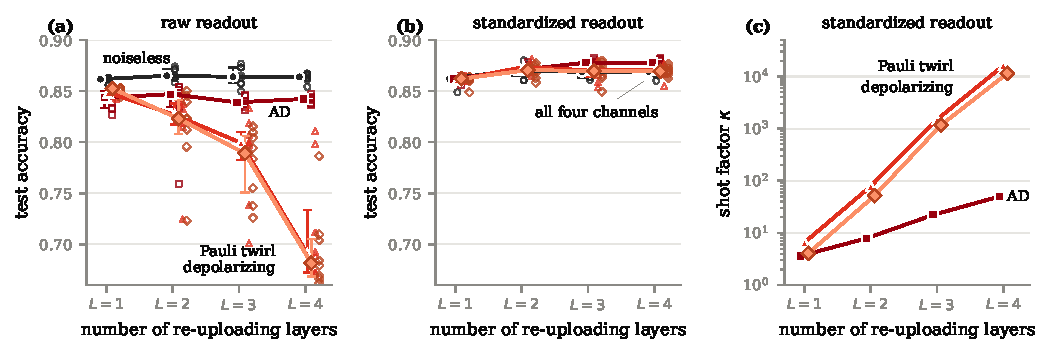
\includegraphics[width=\textwidth]{fig_clf}
\caption{Four-qubit classifier on MNIST against the number of re-uploading
layers. (a) Test accuracy with the raw readout and (b) with the
standardized readout, both after 100 steps, and (c) shot factor $\kappa$ of
Eq.~\eqref{eq:kappa} with the standardized readout. Panels (a) and (b) show the
median and interquartile range over eight initializations, with hollow markers
for the individual runs; one Pauli run at $L=1$ in (b) diverged and lies below
the axis.}
\label{fig:clf}
\end{figure*}

We begin with the simplest way in which noise can change a variational model:
by changing the scale of its output. AD and its Pauli twirl, damping at zero
and at infinite temperature, share the same contraction matrix $T$. Any
difference in scale between them must therefore come from the non-unital vector
$\mathbf t$, which carries the zero-temperature bias (Sec.~\ref{sec:cost}). In this section, we ask
how much of the effect of the noise a trainable output scale can undo, and what
it costs to undo it.

\subsection{Scale and sampling cost}

Consider first the simplest case, in which the noise only rescales and shifts
each expectation value,
\begin{equation}
\tilde z_j=s\,z_j+b_j ,
\label{eq:affine}
\end{equation}
with constants $s\neq0$ and $b_j$ that depend on neither the input nor the
parameters. A trainable affine readout can then undo the noise completely:
every classifier that it can build from the noiseless $\mathbf z$, it
can also build from the noisy $\tilde{\mathbf z}$, so the noise leaves
the model class unchanged. A single qubit under depolarizing noise is an exact
example. Because this channel commutes with every unitary, $N_{\rm ins}$
insertions simply multiply its expectation value $f=\langle Z\rangle$ by a
constant,
\begin{equation}
\tilde f=\lambda_{\rm depol}^{N_{\rm ins}}f ,
\label{eq:depol_scale}
\end{equation}
where $\lambda_{\rm depol}=\frac13(2c+c^2)$ is the factor by which depolarizing
noise shrinks each Bloch component, the average of those of AD.
For anisotropic or non-unital channels, or on more than one qubit, the noisy
model is no longer a rescaled copy of the noiseless one. Whether the scale
still accounts for most of the difference then becomes an empirical question,
which we test in the rest of this section. The average behavior of the spread
on several qubits, its per-layer decay under the twirls and its floor under
AD, is derived in Secs.~\ref{sec:floor} and \ref{sec:pdep}.

On hardware, however, rescaling is not free. The number of shots is one of the
main costs of variational algorithms~\cite{wecker2015progress,gonthier2022measurements},
and an expectation value estimated from $N_s$ shots, $\hat z_j$, has the variance
\begin{equation}
\mathrm{Var}(\hat z_j)=\frac{1-z_j^2}{N_s}\le\frac1{N_s} .
\label{eq:shotvar}
\end{equation}
The standardized readout divides each $z_j$ by its spread $\sigma_j$, so the
shot noise of the standardized $z_j$ has variance
$(1-z_j^2)/(N_s\sigma_j^2)\le1/(N_s\sigma_j^2)$. The smaller the spread, the more
the shot noise is amplified. Keeping the class scores equally precise therefore
requires $N_s\propto1/\sigma^2$, and a channel $\mathcal N$ needs about
$\kappa(\mathcal N)$ times the shots of the noiseless circuit, with the shot
factor
\begin{equation}
\kappa(\mathcal N)=\biggl(\frac{\sigma(\text{None})}{\sigma(\mathcal N)}\biggr)^{2},
\label{eq:kappa}
\end{equation}
where $\sigma$ is the spread $\sigma_j$ at the trained parameters, averaged over
the qubits and the initializations.
In the language of error
mitigation, the trained readout performs a
rescaling~\cite{vovrosh2021simple,urbanek2021mitigating}. Such a rescaling
cannot undo an exponential concentration without an exponential number of
shots~\cite{wang2024errormitigation}. In Sec.~\ref{sec:shots}, we test how well
$\kappa$ predicts the operational shot cost of Sec.~\ref{sec:model_clf}, the
number of shots that a trained classifier actually needs.

The same scale also accounts for the reported smaller gradient magnitudes.
Under Pauli noise, the loss gradients carry the same attenuation factors as the
output~\cite{vanrossum2026biased}. For a rescaled expectation value,
$\partial(s z_j)/\partial\theta=s\,\partial z_j/\partial\theta$, so a trained
output scale restores the size of the gradients. It does not restore their
signal-to-noise ratio under shot noise, which it amplifies by the same factor,
so estimating the gradients to a fixed precision still costs $\kappa$.

\subsection{Classifier}
\label{sec:clf}

We now test this picture in the four-qubit classifier, where the scale
compounds over qubits and layers. With the raw readout and 100 training steps, the unital channels at
first seem to lose trainability as the circuit gets deeper
[Fig.~\ref{fig:clf}(a) and Table~\ref{tab:clf} in Appendix~\ref{app:stats}]. Between $L=1$ and $L=4$, the test
accuracy falls from 0.847 to 0.715 for the Pauli twirl and from 0.851 to 0.695
for depolarizing noise, and the training accuracy falls with it, to 0.700 and
0.672. AD stays at 0.84, and the noiseless circuit at 0.86. Taken at face
value, this would suggest that the non-unital term keeps the deep circuit
trainable.

A closer look shows that the drop comes from the readout, not from the
circuit. If we train the same raw readout for 1000 steps, the unital channels
recover to 0.837 and 0.826 at $L=4$. Over these extra steps, the norm of their
readout weights grows from about 19 to 106 and 109, while for the noiseless
circuit it grows only from 8 to 20. The reason is that, after 100 steps, the
unital channels have shrunk the spread to about 5 and 4 percent of the
noiseless spread, and to below 1 percent before training. With a spread this
small, the raw readout cannot grow its weights fast enough. The circuit itself
remains trainable. With the standardized readout, every channel reaches the
accuracy of the noiseless circuit at every depth [Fig.~\ref{fig:clf}(b)], and
the Pauli and depolarizing channels are statistically indistinguishable from it
(Table~\ref{tab:stats}).

We see the same behavior on Fashion-MNIST at $L=4$. With the raw readout, the
unital channels fall 16 and 17 points below the noiseless circuit (0.765), and
AD falls 5 points below it. With the standardized readout, all three channels
come within two points of the noiseless circuit [Fig.~\ref{fig:fashion} in
Appendix~\ref{app:stats}],
while their shot factors are 34 for AD and $9.9\times10^3$ and
$8.2\times10^3$ for the Pauli and depolarizing channels.

The depolarizing channel at $L=1$ gives an exact check of this picture. Each
$z_j$ then crosses all three noise insertions as a weight-one Pauli string,
so the channel multiplies every $z_j$ by the same factor
$\lambda_{\rm depol}^3$, whatever the parameters. Since the standardized
readout removes a uniform scale, the depolarizing and noiseless classifiers
should make identical predictions, and indeed they do, on every test image. AD
is not a pure rescaling, yet with the standardized readout it too stays within
one percentage point of the noiseless accuracy at every depth
(Table~\ref{tab:stats}).

What the standardized readout cannot remove is the difference in spread
[Fig.~\ref{fig:clf}(c)]. At the end of training, the shot factor of the unital
channels grows by a factor of about 14 per layer, from 4.1 at $L=1$ to
$1.1\times10^4$ at $L=4$ for depolarizing noise and to $1.6\times10^4$ for the
Pauli twirl. For AD, it grows by only about 2.4 per layer, from 3.6 to 50. Note
that the shot factor is not a property of the channel alone. It also depends on
what the model is trained for. With the raw readout, the optimizer moves the
parameters toward less contracted expectation values, and after 1000 steps at $L=4$ the
shot factors are 11 for AD, 320 for the Pauli twirl, and 470 for depolarizing
noise.

In summary, the zero-temperature bias acts in our classifier mainly through
the spread of the expectation values, and the apparent loss of trainability
under the unital channels is a loss of scale. A trained readout absorbs this
loss, but at a cost in shots that grows with depth.

% ============================================================
\section{What the non-unital term changes}
\label{sec:cost}

\begin{figure*}[t]
\centering
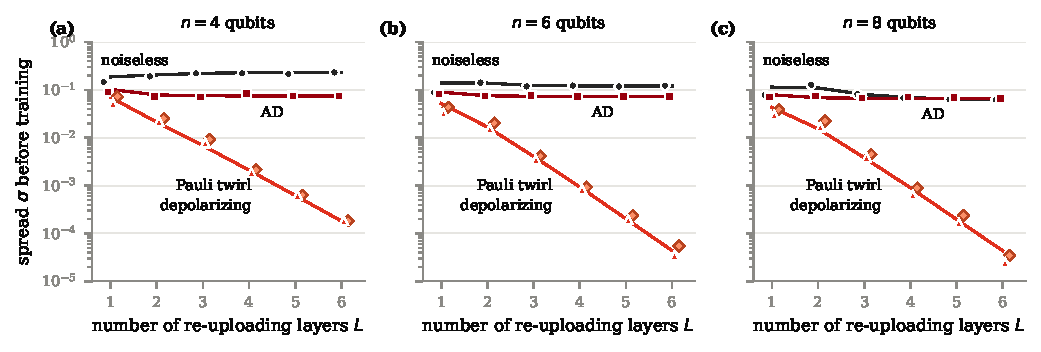
\includegraphics[width=\textwidth]{fig_width}
\caption{Spread $\sigma$ of the expectation values before training against the number of
re-uploading layers at $p=0.3$, for (a) four, (b) six, and (c) eight qubits,
with $n$ principal components as inputs. Markers are the root-mean-square
spread over 300 training images and five parameter draws, shared across depths,
for all four channels. Lines are the exact average over parameters for the
noiseless circuit, AD, and the Pauli twirl (Appendix~\ref{app:width}).}
\label{fig:width}
\end{figure*}

Section~\ref{sec:scale} showed that a trainable scale removes most of the
difference in accuracy between AD and its twirls. AD and its Pauli twirl share
the contraction matrix $T$, so what remains is the non-unital term, of length
$\lVert\mathbf t\rVert=p$. In this section, we show what it changes: the spread of the
expectation values before training, the number of shots needed after training, and how
both depend on the damping strength.

\subsection{Floor of the spread}
\label{sec:floor}

\begin{figure*}[t]
\centering
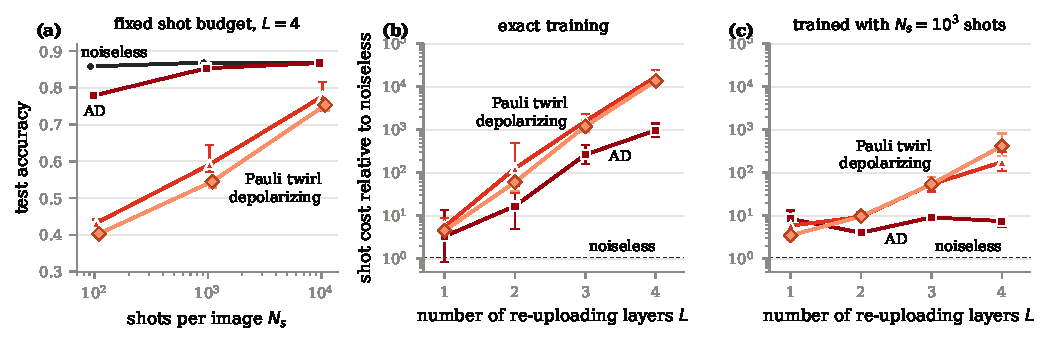
\includegraphics[width=\textwidth]{fig_shots}
\caption{Finite shots in the MNIST classifier at $p=0.3$. (a) Test accuracy at
$L=4$ of models trained and tested with $N_s$ shots per image (median and
interquartile range over eight initializations). (b), (c) Operational shot
cost relative to the noiseless circuit (geometric mean over initializations,
with 95\% bootstrap intervals over initializations) for models trained with
exact expectation values (b) and with $N_s=10^3$ shots (c).}
\label{fig:shots}
\end{figure*}

We start before training, where the effect is cleanest. Here we measure the
spread as
\begin{equation}
\sigma^2=\mathbb E_\theta\,\frac1n\sum_{j=1}^n\mathrm{Var}_{\mathbf a}\,z_j ,
\label{eq:sigma_rms}
\end{equation}
the variance of the $z_j$ over the inputs, averaged over the qubits and over
random parameters, and we write $\sigma_{\AD}$, $\sigma_{\rm Pauli}$, and
$\sigma_{\rm None}$ for its values under AD, the Pauli twirl, and no noise. At
$p=0.3$, the spread separates the channels with both depth and width
(Fig.~\ref{fig:width}). Under the unital channels, the spread shrinks by a nearly constant factor
per layer at every width. Under AD, in contrast, it settles on a floor after
two or three layers. The ratio $\sigma_{\AD}/\sigma_{\rm Pauli}$ therefore
grows geometrically, by a factor of about 3.3 per layer at $n=4$, and its
square, which is the ratio of their shot factors, grows by about 11 per layer.
As the circuit gets wider,
the noiseless spread falls, as expected for a scrambling circuit, but the floor
barely moves. At $n=8$ and $L\ge4$, the AD spread is therefore as large as
the noiseless one.

The floor comes from the
non-unital term. To see this, consider a $Z$ component propagated backward
from the readout. Under AD it becomes $c^2Z+t_zI$, with $t_z=p$, whereas the
Pauli twirl keeps only $c^2Z$. The identity part behaves very differently from
the rest. Its expectation value is 1 in every state, so it reaches the readout
no matter what the earlier layers do. The twirl has no such part, and every
component keeps shrinking from layer to layer. Under AD, the damping after the last entangler
branches the $Z$ component of each $z_j$ into the identity and adds
\begin{equation}
\delta z_j=p(1-p)\bigl[(1-p)\,v_z\cos a_j-c\,v_y\sin a_j\bigr]
\label{eq:floor}
\end{equation}
to $z_j$, where $(v_x,v_y,v_z)$ is the direction into which the final
trainable block rotates $Z_j$. Averaging over the parameters,
we obtain a closed form for this last-layer
contribution,
\begin{multline}
\sigma_\infty^2=\frac{p^2(1-p)^2}{n}\sum_j\Bigl[\frac{(1-p)^2}{2}\,
\mathrm{Var}(\cos a_j)\\
+\frac{1-p}{4}\,\mathrm{Var}(\sin a_j)\Bigr],
\label{eq:floor_var}
\end{multline}
which at $p=0.3$ matches the floor of the AD spread to within 0.5\% for $n\ge4$.

This floor fits well with what is
known about noise-induced concentration. Unital noise concentrates local
expectation values exponentially in
depth~\cite{wang2021noiseinduced,schumann2024emergence}. Under non-unital
noise, by contrast, the variance of local expectation values over random
circuits stays bounded from below by an amount set by the non-unital
term~\cite{mele2026noise}. Equation~\eqref{eq:floor_var} is the counterpart of
that bound for the variance over inputs. After the average over parameters,
branchings in different layers are uncorrelated, so
$\sigma_{\AD}^2\ge\sigma_\infty^2$ at every depth. Both bounds scale as
$\lVert\mathbf t\rVert^2=p^2$ and do not decay with depth. At weak damping, the
branchings of earlier layers raise the floor above this bound, as we show in
Sec.~\ref{sec:pdep}. At $p=0.3$, however, the last
layer alone sets the spread under AD. This is in line with the
effective shallowness of noisy circuits~\cite{mele2026noise}: only the last few
layers before the readout shape the output.

The floor also shows how the zero-temperature bias
depends on temperature. At finite temperature, the damping of a qubit with
splitting $\hbar\omega$ relaxes toward the thermal excited-state population
$N=(e^{\hbar\omega/k_BT}+1)^{-1}$, and Sec.~\ref{sec:channels} gives
\begin{equation}
t_z=p(1-2N)=p\tanh\frac{\hbar\omega}{2k_BT}
\label{eq:tz}
\end{equation}
at fixed $p$, that is, at fixed measured $T_1$. At fixed coupling to the bath,
$1/T_1$ itself grows as $\coth(\hbar\omega/2k_BT)$. At weak damping, $t_z$ is
then independent of temperature to first order in $p$, and the temperature
acts through the contraction instead. At fixed $T_1$, the picture is simple. The last-layer term,
Eq.~\eqref{eq:floor}, is linear in $t_z$, so it scales exactly as $1-2N$.
Strings of higher Pauli weight can branch into the identity on several qubits
and add higher powers of $t_z$, but in the exact average over parameters they
change this scaling by less than half a percent.
The floor therefore vanishes linearly in $1-2N$
as the temperature rises, and it reaches zero at the Pauli twirl,
$N=\frac12$.

\subsection{Sampling cost}
\label{sec:shots}

\begin{figure*}[t]
\centering
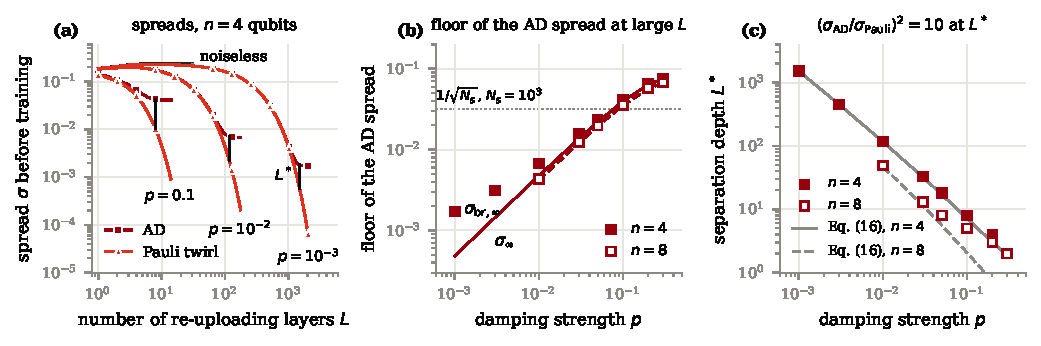
\includegraphics[width=\textwidth]{fig_sep}
\caption{Dependence of the separation on the damping strength, from the exact
average over parameters before training (5000 image pairs at $n=4$, 700 at
$n=8$). (a) Spread against depth at $n=4$ for AD (squares) and the
Pauli twirl (triangles) at three values of $p$, and for the noiseless circuit
up to $L=30$; vertical segments mark $L^*$. (b) Floor $\sigma_{\rm br,\infty}$
of the AD spread (markers) and its last-layer part $\sigma_\infty$
[Eq.~\eqref{eq:floor_var}, lines] for $n=4$ (filled, solid) and $n=8$ (hollow,
dashed); the dotted line is the shot noise $1/\sqrt{N_s}$ at $N_s=10^3$.
(c) Separation depth $L^*$ (markers) and Eq.~\eqref{eq:Lstar} (gray lines).
At $n=8$ the exact average was computed for $p\ge0.01$.}
\label{fig:sep}
\end{figure*}

We next test whether the shot factor predicts the number of shots that a
trained classifier actually needs, by comparing it with the operational shot
cost of Sec.~\ref{sec:model_clf}. After training with exact expectation values,
this cost follows $\kappa$ for the unital channels but not for AD
[Fig.~\ref{fig:shots}(b) and Table~\ref{tab:pdep_trained}]. At $L=4$, AD needs
19 times more shots than its shot factor predicts. Even so, the Pauli twirl
still needs 18 times the shots of AD. The extra cost of AD comes from the
readout. The shot factor only looks at the average spread of the $z_j$, whereas
the readout amplifies the shot noise of each $z_j$ by its own weight. Exact
training lets the AD readout rely on expectation values whose spread is far
smaller than in the noiseless circuit. We capture this effect with the
readout-weighted noise gain
$G=\bigl\langle\sum_j\lVert\mathbf w_j\rVert^2(1-z_j^2)/\sigma_j^2\bigr\rangle$,
where $\mathbf w_j$ is the column of $W$ that multiplies $z_j$ and the average
runs over the test images. If the shot noise of different qubits is
uncorrelated, $G$ is $N_s$ times the total shot-noise variance of the class
scores. It reproduces the measured cost ratios to within a factor of 1.6 for
$L\ge2$ (Table~\ref{tab:gain} in Appendix~\ref{app:stats}).

The picture changes when we also train under shot noise
[Fig.~\ref{fig:shots}(a) and (c)]. Trained and tested with $10^3$ shots per
image, AD stays within 1.5 percentage points of the noiseless accuracy at every
depth, while the twirled channels lose up to 33 points at $L=4$. Part of this
loss already arises in training. Evaluated without shot noise, the twirled
models trained with shots remain clearly less accurate than those trained
exactly, whereas AD loses almost nothing. After training with shots, the
operational cost of AD stays close to its shot factor, whereas for the twirls
it still grows by a factor of 3 to 5 per layer [Fig.~\ref{fig:shots}(c)]. The
reason is that training under shot noise moves the circuit toward expectation
values whose spread exceeds the shot noise $1/\sqrt{N_s}$. Under AD, the
smallest spread rises to the floor of Fig.~\ref{fig:width}, above the shot
noise, while under the twirls it stays below it (Appendix~\ref{app:stats}).

Finally, the learned rescaling is far
cheaper than generic error mitigation. Probabilistic error
cancellation~\cite{temme2017error} of the twirled channel would multiply the
shots by $(1-p)^{-2}$ per insertion, or $(1-p)^{-72}\approx10^{11}$ over the 36
insertions of the $L=4$ classifier, consistent with the exponential lower
bounds on mitigation~\cite{takagi2023universal,quek2024exponentially}. The
rescaling learned under shot noise, by comparison, needs at most 417 times the
shots of the noiseless circuit. It restores, however, only the spread of the few
expectation values that the task uses, not the noiseless state.

\subsection{Dependence on the damping strength}
\label{sec:pdep}

\begin{table}[t]
\caption{Dependence on the damping strength $p$ before training, from the
exact average over parameters: the depth $L^*$ at which
$(\sigma_{\AD}/\sigma_{\rm Pauli})^2$ first reaches 10, the floor
$\sigma_{\rm br,\infty}$ of the AD spread and its last-layer part $\sigma_\infty$
[Eq.~\eqref{eq:floor_var}], and the number of shots
$1/\sigma_{\rm br,\infty}^2$ that resolves the floor. The floor is estimated from 5000 ($n=4$) and 700 ($n=8$) random image pairs, with a sampling error of about 1\%.}
\label{tab:pdep}
\begin{ruledtabular}
\begin{tabular}{lccccc}
 & \multicolumn{4}{c}{$n=4$} & $n=8$\\
$p$ & $L^*$ & $\sigma_{\rm br,\infty}$ & $\sigma_\infty$ & $1/\sigma_{\rm br,\infty}^2$ & $L^*$\\
\colrule
0.001 & 1508 & 0.0017 & 0.0005 & $3.4\times10^5$ & --\\
0.003 & 453 & 0.0031 & 0.0014 & $1.0\times10^5$ & --\\
0.01 & 117 & 0.0067 & 0.0047 & $2.2\times10^4$ & 49\\
0.03 & 33 & 0.0155 & 0.0137 & $4.2\times10^3$ & 13\\
0.05 & 18 & 0.0235 & 0.0219 & $1.8\times10^3$ & 8\\
0.1 & 8 & 0.0408 & 0.0396 & 600 & 5\\
0.2 & 4 & 0.0647 & 0.0637 & 240 & 3\\
0.3 & 2 & 0.0757 & 0.0747 & 170 & 2\\
\end{tabular}
\end{ruledtabular}
\end{table}

So far we have worked at strong damping, $p=0.3$. We now turn to weaker
damping, closer to current hardware, where both sides of the comparison change
with $p$ (Table~\ref{tab:pdep} and Fig.~\ref{fig:sep}). At weak damping,
the twirled spread decays per layer as $e^{-np}$. This is because a scrambled
Pauli string has about $3n/4$ non-identity sites, and each of the two
insertions per layer shrinks such a site by a factor of about $1-2p/3$ on
average. The floor of the AD spread, $\sigma_{\rm br,\infty}$, changes as well.
Its square has two parts,
$\sigma_{\rm br,\infty}^2\approx\sigma_\infty^2+b_{\rm br}\,p$. The first is
proportional to $p^2$ [Eq.~\eqref{eq:floor_var}]. The second comes from
branchings in the roughly $1/(np)$ earlier layers that the damping does not yet
suppress. It acts on the input dependence of those layers, which concentrates
with width, so $b_{\rm br}$ falls by about an order of magnitude from $n=4$ to
$n=8$.

To quantify when the two spreads separate, we define the separation depth
$L^*$ as the depth at which $(\sigma_{\AD}/\sigma_{\rm Pauli})^2$ first
reaches 10 (Table~\ref{tab:pdep}). There, the twirl needs ten times the shots
of AD before training. Since the AD spread splits into the twirled part
and a branching part $\sigma_{\rm br}$ (Appendix~\ref{app:width}),
\begin{equation}
\sigma_{\AD}^2=\sigma_{\rm Pauli}^2+\sigma_{\rm br}^2 ,
\label{eq:split}
\end{equation}
this happens when $\sigma_{\rm br}=3\,\sigma_{\rm Pauli}$. With
$\sigma_{\rm br}\approx\sigma_{\rm br,\infty}$ and
$\sigma_{\rm Pauli}\approx\sigma_{\rm None}\,e^{-npL}$, we obtain the estimate
\begin{equation}
L^*\approx\frac{1}{np}\,\ln\frac{3\,\sigma_{\rm None}}{\sigma_{\rm br,\infty}},
\label{eq:Lstar}
\end{equation}
where $\sigma_{\rm None}$ is taken at large depth (0.24 at $n=4$ and 0.062 at
$n=8$). At weak damping, this estimate agrees closely with the exact separation
depth [Fig.~\ref{fig:sep}(c)], and it grows
roughly as $p^{-1}\ln(1/p)$. Interestingly, at fixed weak damping $L^*$ falls
faster than $1/n$ (Table~\ref{tab:pdep}). This is because the noiseless spread
in the logarithm concentrates with width faster than the floor does.

This has a clear consequence for real devices. On superconducting hardware,
the damping
is of order $10^{-3}$ per two-qubit gate, for gate times of 30 to 400~ns and
$T_1$ of order $100~\mu$s~\cite{krantz2019quantum}. In our model, one of the
two insertions per layer follows a ring of $n$ CNOTs, so $p$ per insertion
corresponds to several gate durations. At $p=10^{-3}$, the separation needs
about 1500 layers at $n=4$ (Table~\ref{tab:pdep}). The difference in
spread between AD and its twirls is therefore a property of strong damping or
of very deep circuits.

\begin{table*}[t]
\caption{Trained classifiers at weaker damping (MNIST, standardized readout,
exact expectation values, eight initializations): test accuracy (mean $\pm$ SD), operational
shot cost relative to the noiseless circuit at the same depth, shot factor
$\kappa$, and the squared ratio of the AD and Pauli-twirl spreads before
training, $(\sigma_{\AD}/\sigma_{\rm Pauli})^2$, from the exact average over
parameters of Table~\ref{tab:pdep}. The row $p=0.3$ repeats
Secs.~\ref{sec:clf} and \ref{sec:shots}.}
\label{tab:pdep_trained}
\begin{ruledtabular}
\begin{tabular}{llccccccccccc}
 & & \multicolumn{4}{c}{test accuracy} & \multicolumn{3}{c}{shot cost / noiseless} & \multicolumn{3}{c}{$\kappa$} & before\\
$p$ & $L$ & None & AD & Pauli & Depol & AD & Pauli & Depol & AD & Pauli & Depol & training\\
\colrule
0.3 & 4 & $.869\pm.005$ & $.876\pm.005$ & $.870\pm.007$ & $.870\pm.004$ & 967 & $1.7\times10^4$ & $1.4\times10^4$ & 50 & $1.6\times10^4$ & $1.1\times10^4$ & $1.3\times10^3$\\
0.05 & 4 & $.869\pm.005$ & $.866\pm.005$ & $.866\pm.007$ & $.864\pm.004$ & 4.7 & 4.8 & 4.1 & 4.6 & 4.7 & 4.4 & 1.06\\
0.1 & 4 & $.869\pm.005$ & $.872\pm.005$ & $.863\pm.004$ & $.863\pm.003$ & 13.1 & 21.5 & 14.9 & 15.6 & 21.2 & 17.5 & 1.69\\
0.1 & 8 & $.831\pm.012$ & $.866\pm.006$ & $.840\pm.009$ & $.838\pm.007$ & 115 & 466 & 495 & 62 & 484 & 459 & 16.8\\
\end{tabular}
\end{ruledtabular}
\end{table*}

Trained classifiers follow this picture (Table~\ref{tab:pdep_trained}). Well
below the separation depth, at $p=0.05$ and $L=4$ ($L^*=18$), AD and its twirls
reach the same accuracy at nearly the same shot cost, as $\kappa$ predicts.
Closer to it, at $p=0.1$ and $L=4$ ($L^*=8$), the twirls already need more shots
than AD. At $L=L^*=8$, the channels finally separate. The twirls then need
about four times the shots of AD, in the same direction as the spread ratios
before and after training. At this depth, AD is also 2.6 points more accurate
than the Pauli twirl. It is not, however, more accurate than the best noiseless
circuit (0.869 at $L=2$ to 4), and with $10^3$ shots per image it falls behind
the noiseless circuit (Appendix~\ref{app:stats}).

% ============================================================
\section{Conclusion}
\label{sec:conclusion}

We have compared amplitude damping with its twirls, in particular with the
Pauli twirl, which is damping at infinite temperature. In our classifier, the
zero-temperature bias acts mainly through the spread of the expectation values.
Under AD, the spread stops at a floor fixed at strong damping by the last layer,
and at fixed $T_1$ this floor falls linearly in $1-2N$ as the temperature
rises. Under the twirls, it keeps shrinking by a constant factor per layer at
every width up to eight qubits.

Training an output scale removes most of the resulting differences in accuracy
in exact simulation. What it removes reappears as a sampling cost. With $10^3$
shots per image at $p=0.3$, the classifier under AD stays within 1.5 percentage
points of the noiseless accuracy at depths 1 to 4, while the twirled
classifiers lose up to 33 points at four layers. The separation needs a depth
that grows roughly as $(np)^{-1}\ln(1/p)$, about 1500 layers on four qubits at
$p=10^{-3}$, so it matters only at strong damping or in very deep circuits.
This gives a simple reading of the reported degradation under
twirling. The twirls shrink the scale at which the outputs must be read, more
than they reduce what the model can learn.

Our results suggest a practice for comparing noise structures in variational
models. A comparison should report the output scale, or train one, together
with the shot budget it implies. Without the scale, a difference in accuracy
can reflect the readout rather than the circuit. Without the shot budget, a
trained scale hides the cost of the noise.

Several questions remain open. Our simulations are exact and small. We
established the width dependence before training, up to eight qubits, but
training beyond four qubits was out of reach of exact simulation, and our shot
model in training neglects the correlations between qubits. It also remains
to be seen whether trained models follow the temperature dependence of the
floor, and whether the results hold on hardware, where damping comes with
dephasing.

\begin{acknowledgments}

We thank Vietnam National University Ho Chi Minh City (VNU-HCM) for its support.
Claude Opus 5.5 (Anthropic) assisted with the research and the drafting of the
manuscript.

\end{acknowledgments}

\section*{Data availability}
The code, the result files, and the scripts that reproduce every number and
figure in this paper are available at
\url{https://github.com/Identity-Operator/zero-vs-infinite-T-damping} and archived
on Zenodo at \href{https://doi.org/10.5281/zenodo.23053251}{doi:10.5281/zenodo.23053251}~\cite{nguyen2026zenodo}.

% ============================================================
\appendix

\section{Statistical tests}
\label{app:stats}

\begin{table}[t]
\caption{Standardized-readout classifier on MNIST: difference from the
noiseless circuit in test accuracy. $P$ values from paired $t$ tests over the
eight initializations, Holm-adjusted over the 11 tests of the table.}
\label{tab:stats}
\begin{ruledtabular}
\begin{tabular}{llccc}
$L$ & channel & $\Delta$acc & 95\% CI & $P$\\
\colrule
1 & AD & $+0.001$ & $[-0.003,+0.005]$ & 1\\
1 & Pauli & $-0.059$ & $[-0.178,+0.001]$ & 1\\
1 & Depol & $0$ & exact & --\\
2 & AD & $+0.003$ & $[-0.003,+0.009]$ & 1\\
2 & Pauli & $+0.004$ & $[-0.003,+0.010]$ & 1\\
2 & Depol & $+0.000$ & $[-0.004,+0.004]$ & 1\\
3 & AD & $+0.009$ & $[+0.003,+0.015]$ & 0.02\\
3 & Pauli & $+0.001$ & $[-0.007,+0.008]$ & 1\\
3 & Depol & $+0.000$ & $[-0.007,+0.007]$ & 1\\
4 & AD & $+0.008$ & $[+0.002,+0.013]$ & 0.004\\
4 & Pauli & $+0.001$ & $[-0.007,+0.009]$ & 1\\
4 & Depol & $+0.001$ & $[-0.006,+0.008]$ & 1\\
\end{tabular}
\end{ruledtabular}
\end{table}

\begin{table*}[t]
\caption{Test accuracy of the classifier on 3037 MNIST images (mean $\pm$ SD
over eight initializations) against the number of re-uploading layers $L$.
The raw readout is trained for 100 steps and, at $L=4$, for 1000 steps; the
standardized readout of Eq.~\eqref{eq:readout} for 100 steps.
$^\dagger$One of the eight runs diverged (test accuracy 0.382); the other seven
lie between 0.860 and 0.865.}
\label{tab:clf}
\begin{ruledtabular}
\begin{tabular}{lccccccccc}
 & \multicolumn{5}{c}{raw readout} & \multicolumn{4}{c}{standardized readout}\\
 & $L=1$ & $L=2$ & $L=3$ & $L=4$ & $L=4$, 1000 steps & $L=1$ & $L=2$ & $L=3$ & $L=4$\\
\colrule
None & $.861\pm.003$ & $.866\pm.005$ & $.865\pm.009$ & $.863\pm.004$ & $.862\pm.007$ & $.860\pm.005$ & $.869\pm.007$ & $.868\pm.006$ & $.869\pm.005$\\
AD & $.842\pm.010$ & $.835\pm.032$ & $.839\pm.005$ & $.841\pm.004$ & $.872\pm.003$ & $.861\pm.003$ & $.872\pm.003$ & $.877\pm.004$ & $.876\pm.005$\\
Pauli & $.847\pm.003$ & $.817\pm.039$ & $.787\pm.044$ & $.715\pm.057$ & $.837\pm.013$ & $.802\pm.170^\dagger$ & $.873\pm.005$ & $.869\pm.009$ & $.870\pm.007$\\
Depol & $.851\pm.003$ & $.814\pm.041$ & $.778\pm.034$ & $.695\pm.041$ & $.826\pm.012$ & $.860\pm.005$ & $.869\pm.006$ & $.869\pm.010$ & $.870\pm.004$\\
\end{tabular}
\end{ruledtabular}
\end{table*}

We collect here the hypothesis tests behind the comparisons in the main text.
Classifier results are given as the mean and standard deviation (SD) over
eight initializations with fixed data. Because all runs share one finite test
set, a difference between two conditions is uncertain through both the
initializations and the test images. Accuracy differences therefore come with
a 95\% confidence interval (CI) from a two-level
bootstrap~\cite{efron1994introduction} ($2\times10^4$ resamples) that
resamples both, with the initializations resampled jointly for the two
conditions since they share their initial parameters. They also come with the
$P$ value of the paired $t$ test across the eight initializations. To avoid
confusion with the noise strength $p$, we denote $P$ values by a capital $P$. The $P$ values of
Table~\ref{tab:stats} are Holm-adjusted over its 11 tests. Two remain below
0.05, both for AD, at $L=3$ and 4.

\begin{figure*}[t]
\centering
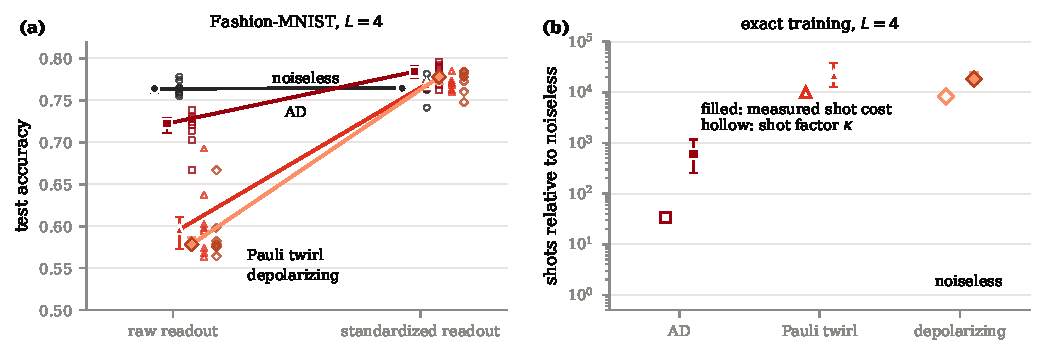
\includegraphics[width=\textwidth]{fig_fashion}
\caption{Four-qubit classifier on Fashion-MNIST at $L=4$ and $p=0.3$. (a) Test
accuracy with the raw and the standardized readout, as the median and
interquartile range over eight initializations, with each run as a hollow
marker. (b) Shot factor $\kappa$ (hollow) and operational shot cost relative to
the noiseless circuit (filled; geometric mean over initializations with 95\%
bootstrap intervals), both after exact training.}
\label{fig:fashion}
\end{figure*}

\paragraph{Classifier on Fashion-MNIST.}
These results are shown in Fig.~\ref{fig:fashion}. At $L=4$, the differences from the noiseless circuit are $+0.017$, CI
$[+0.007,+0.029]$, $P=0.03$, for AD; $+0.005$, CI $[-0.004,+0.014]$, $P=0.28$,
for the Pauli twirl; and $+0.009$, CI $[-0.0001,+0.018]$, $P=0.08$, for
depolarizing noise (paired $t$, Holm-adjusted over the three channels).

\paragraph{Shot cost.}
At $L=4$ with exact training, the operational shot cost of AD exceeds its shot
factor 19-fold, with a 95\% bootstrap interval over initializations of 12 to
30. The Pauli twirl needs 18 times the shots of AD on MNIST (10 to 29) and 36
times on Fashion-MNIST (17 to 85). Trained and tested with $10^3$ shots, AD lies 0.7, 0.9, 1.2, and 1.5 points
below the noiseless accuracy at $L=1$ to 4, and at $L=4$ it stays within 1.5
points also with $10^4$ shots. Evaluated with exact expectation values, the
twirled models trained with $10^3$ shots are about 0.11 less accurate than
those trained exactly, and AD about 0.01. At $L=4$ and $N_s=10^3$, the geometric
mean of the smallest spread is 0.075 for AD, compared with 0.0065 under exact
training and 0.24 for the noiseless circuit, and 0.005 and 0.003 for the Pauli and depolarizing channels. Table~\ref{tab:gain} compares the exact-training costs
with the noise gain $G$ of Sec.~\ref{sec:shots} and with the shot factor.

\begin{table*}[t]
\caption{Readout-weighted noise gain $G$ of Sec.~\ref{sec:shots} compared with the
operational shot cost of the classifiers trained with exact expectation values at
$p=0.3$. All entries are relative to the noiseless circuit and are geometric means
over initializations. For $L\ge2$, $G$ matches the shot cost to within a factor of
1.6, whereas the shot factor $\kappa$ underestimates the cost of AD by up to 19 times.}
\label{tab:gain}
\begin{ruledtabular}
\begin{tabular}{llrrrrrrrrr}
 & & \multicolumn{3}{c}{shot cost / noiseless} & \multicolumn{3}{c}{$G/G_{\rm None}$} & \multicolumn{3}{c}{$\kappa$}\\
dataset & $L$ & AD & Pauli & Depol & AD & Pauli & Depol & AD & Pauli & Depol\\
\colrule
MNIST & 1 & 3.3 & 5.6 & 4.5 & 0.9 & 1.3 & 4.3 & 3.6 & 6.5 & 4.1\\
MNIST & 2 & 17 & 125 & 60 & 14 & 125 & 58 & 7.9 & 79 & 52\\
MNIST & 3 & 263 & $1.6\times10^3$ & $1.2\times10^3$ & 277 & $2.0\times10^3$ & $1.6\times10^3$ & 22 & $1.5\times10^3$ & $1.2\times10^3$\\
MNIST & 4 & 967 & $1.7\times10^4$ & $1.4\times10^4$ & 983 & $2.4\times10^4$ & $1.5\times10^4$ & 50 & $1.6\times10^4$ & $1.1\times10^4$\\
Fashion-MNIST & 4 & 603 & $2.2\times10^4$ & $1.8\times10^4$ & 400 & $1.6\times10^4$ & $1.2\times10^4$ & 34 & $9.9\times10^3$ & $8.2\times10^3$\\
\end{tabular}
\end{ruledtabular}
\end{table*}

\paragraph{Weaker damping.}
At $p=0.1$ and $L=8$ (Table~\ref{tab:pdep_trained}), AD minus the Pauli twirl
in accuracy is $+0.026$, CI $[+0.017,+0.035]$. Evaluated with $10^3$ shots per
image, AD reaches 0.69 against 0.83 for the noiseless circuit.

\section{Spread before training}
\label{app:width}

The lines in Fig.~\ref{fig:width} are exact averages, over parameters drawn
uniformly from $[0,2\pi)$, of Eq.~\eqref{eq:sigma_rms}, where the variance
runs over the first 300 training images. We compute them in
the Heisenberg picture from the second moments of the Pauli-string
coefficients of $Z_j$, with the parameters shared between two images. Every
uniformly random $R_ZR_YR_Z$ block removes the cross moments between different
strings because, averaged over its angles, the entries $R_{bc}$ of its
adjoint action have vanishing first moments and different columns are
uncorrelated, $\mathbb E_\theta[R_{ab}R_{a'c}]=0$ for $b\neq c$. Between two
blocks the circuit acts site by site (channel, $R_X(a_j)$, channel), so the
second moments of two images propagate through the elementwise product of the
two composite site maps, followed by the entangling ring, which permutes the
strings up to a sign. The second moments therefore obey a closed recursion, which is exact up
to the sampling of image pairs: all pairs for $n\le5$, and 5000 random pairs
for $n\ge6$. Against brute-force averages of the density-matrix simulation,
the recursion agrees within one to two standard errors in all 18 cells at
$n=2$ and 3 and $L=1$ to 3. An independent density-matrix simulation at $n=4$, with 200 parameter draws, agrees within two standard errors in all 12 cells for the noiseless circuit, AD, and the Pauli twirl at $L=1$ to 4, and in all four cells for AD and the Pauli twirl at $p=0.1$ and $L=4$ and 8.

Under AD the adjoint channel maps $Z$ to $c^2Z+pI$. The next random block
averages the cross moments between the $I$ and $Z$ branches to zero, which
gives Eq.~\eqref{eq:split}, with $\sigma_{\rm br}$ collecting the paths through
at least one branching into the identity. The
branching after the last entangler gives Eq.~\eqref{eq:floor}. Averaged over
the final block, with $\mathbb E\,v_z^2=\frac12$, $\mathbb E\,v_y^2=\frac14$, and
$\mathbb E\,v_zv_y=0$, it yields Eq.~\eqref{eq:floor_var}. The agreement
within 0.5\% quoted in Sec.~\ref{sec:floor} uses all image pairs.
Branchings in earlier layers are attenuated by the rest of the circuit. At
weaker damping they are not, and they add the term $b_{\rm br}\,p$ of
Sec.~\ref{sec:pdep}. For uniformly
distributed angles, $\sigma_\infty=0.096$. The measured points in
Fig.~\ref{fig:width} use five parameter draws, the same parameter vectors at
every depth (those of depth $L$ are the leading entries of those of depth 6),
so their deviations are correlated across $L$. The distribution over the
parameters is heavy-tailed, and five draws tend to fall below the average, as
for the Pauli twirl at $n=8$ and $L\ge4$. An independent Pauli-path simulation
reproduces these five draws to $2\times10^{-12}$ and, over 120 further draws
at $L=4$, agrees with the exact average within one standard error.

In this exact average, the per-layer growth of the ratio of the AD and
Pauli-twirl spreads, 3.3 at $n=4$ (Sec.~\ref{sec:floor}), rises to 4.5 for
$n\ge6$, and that of its square from 11 to 20. At $n=4$, the squared ratio is
2.1 at $L=1$ and $1.3\times10^3$ at $L=4$. The per-layer decay rate of the
twirled spread agrees with $np$ within 1\% for $p\le0.05$ at $n=4$ and 8. For
$p\le0.03$ the coefficient $b_{\rm br}$ of Sec.~\ref{sec:pdep} is
$(1.8$--$2.7)\times10^{-3}$ at $n=4$ and $(1.0$--$2.4)\times10^{-4}$ at $n=8$, and
Eq.~\eqref{eq:Lstar} agrees with the exact separation depth within 1\% for
$p\le0.01$ and within one layer for larger $p$ at $n=4$, and within two layers
for $p\le0.03$ at $n=8$. At finite temperature, the branching part of the
spread at $n=4$ follows $1-2N$ within 0.4\% for every $N\le\frac12$ and
$L\le8$ at $p=0.3$, and within 0.2\% at $p=0.1$.

\section{Training details and numerical checks}
\label{app:training}

\paragraph{Classifier training.}
To prepare the inputs, we standardize the pixel values, compute four principal
components, and map each component linearly to an angle, sending its minimum
to 0 and its maximum to $2\pi$. The standardization, the principal components,
and the extrema are fitted on 1000 training images and applied unchanged to all
3037 test images of the three digits. Training minimizes the softmax cross-entropy with Adam~\cite{kingma2014adam} at
learning rate $0.05$ for 100 full-batch steps unless stated otherwise, without
weight decay. The circuit angles start uniformly in $[0,2\pi)$, the readout
weights from a zero-mean normal distribution with standard deviation 0.5, and
the bias at zero. The density matrix
is simulated exactly in PyTorch~\cite{paszke2019pytorch}. No regularizing
constant is added to $\boldsymbol\sigma$ in the standardized readout. In one
run, the spread of one $z_j$ fell to $5\times10^{-5}$, and the training diverged
(Table~\ref{tab:clf}). The Fashion-MNIST classes are T-shirt, pullover, and
coat, with 3000 test images. For reference, logistic regression, a
$k$-nearest-neighbor classifier ($k=15$), and a support-vector machine with a
radial kernel, trained on the same angles, reach 0.856, 0.879, and 0.886 on
MNIST and 0.733, 0.758, and 0.748 on Fashion-MNIST.

\paragraph{Shot model.}
For the finite-shot runs, each image is measured $N_s$ times in the
computational basis, and the estimate $\hat z_j$ of Eq.~\eqref{eq:shotvar} is the
mean of the outcomes $\pm1$ of qubit $j$. At test time we sample the outcomes from the exact distribution of
the measured state, five times per model, and in every draw we re-estimate
$\boldsymbol\mu$ and $\boldsymbol\sigma$ from $N_s$ shots of each training
image, as one would on hardware. In training we replace each $z_j$ by
\begin{equation}
\hat z_j=z_j+\sqrt{\frac{1-z_j^2}{N_s}}\;\varepsilon_j ,
\label{eq:shot_train}
\end{equation}
where $\varepsilon_j$ is a standard normal random number, redrawn at every step
and for every image, and compute $\boldsymbol\mu$ and
$\boldsymbol\sigma$ from the noisy $\hat z_j$; gradients flow through $z_j$. This
Gaussian model has the exact shot variance of each $z_j$ but neglects the
correlations between qubits and the shot noise of parameter-shift gradients. We train with
$N_s=10^3$ at $L=1$ to 4, and with $N_s=10^2$ and $10^4$ at $L=4$. The
operational shot cost is interpolated in $\log N_s$ on a grid from 10 to
$10^8$. It is undefined for three exactly trained models at $L=1$, which we
omit: the diverged Pauli run, and one noiseless and one depolarizing model
whose accuracy stays more than 0.01 below its exact value up to $10^8$ shots.

\bibliography{refs}

\end{document}
